\documentclass[runningheads]{llncs}
%
\usepackage[T1]{fontenc}
\usepackage{graphicx}


\begin{document}
%
\title{Contribution Title}
%
%\titlerunning{Abbreviated paper title}
% If the paper title is too long for the running head, you can set
% an abbreviated paper title here
%
\author{First Author\inst{1}\orcidID{0000-1111-2222-3333} \and
Second Author\inst{2,3}\orcidID{1111-2222-3333-4444} \and
Third Author\inst{3}\orcidID{2222--3333-4444-5555}}
%
\authorrunning{F. Author et al.}
% First names are abbreviated in the running head.
% If there are more than two authors, 'et al.' is used.
%
\institute{Princeton University, Princeton NJ 08544, USA \and
Springer Heidelberg, Tiergartenstr. 17, 69121 Heidelberg, Germany
\email{lncs@springer.com}\\
\url{http://www.springer.com/gp/computer-science/lncs} \and
ABC Institute, Rupert-Karls-University Heidelberg, Heidelberg, Germany\\
\email{\{abc,lncs\}@uni-heidelberg.de}}
%
\maketitle
%
\begin{abstract}
	...

\keywords{First keyword  \and Second keyword \and Another keyword.}
\end{abstract}


\section{Introduction}
\label{sec:introduction}



% ############################# %
% Espace réservé aux encadrants %
% ############################# %



\section{Modèle informel}
\label{sec:informal-model}


\newpage

\section{Modèle formel}
\label{sec:formal-model}

\subsection{Mosélisation d'une liste d'odre}

La modélisation de notre liste d'ordre doit prendre en compte les besoins et contraintes évoqués plus haut.
Pour cela, nous avons choisi de la représenter comme cela : $O = \{\Gamma, R\}$, avec $\Gamma$ l'ensemble des trains et $R$ notre régulateur.
Chaque train peut être représenté par un identifiant unique, une position, une direction et son programme : $t = (id, pos, dir, P)$, avec $t \in \Gamma$.
Le régulateur, portant une grande partie de la logique du modèle, se représente de manière plus complexe : $R = (E,T,S,W,G,H,TL)$.
%##########
%Définit ce qu'est un event à ce moment ou plus haut ?
%##########
Nous ne détaillerons pas l'ensemble des éléments de $R$ ici, mais nous pouvons en donner un aperçu rapide : $E$ contient l'ensemble des events,
$T$ le token courant pour chaque ressource et $H$ la dernière position connue de chaque train par le régulateur.

Idée: Pourquoi besoin des jetons ? Plusieurs trains peuvent attendre la même ressource critique, il faut donc créer un "ordre de passage".
Avoir un unique token par ressource complexifie les règles.

\subsection{Détecter les problèmes}
Cette section est particulièrement importante, modéliser les problèmes que l'on peut rencontrer permet de les détecter.
Cette phrase peut paraître évidente, mais elle est centrale dans notre méthodologie. Ici, nous pouvons faire face à deux problèmes : 
les trains n'arrivent pas destination, c'est un deadlock, ou les trains partage une même ressource, c'est un crash. 
Point important, nos règles de transitions se basent sur l'interleaving, les trains ne peuvent donc pas se croiser. (($\triangle$,2)->($\triangle$,3) || ($O$,3)->($O$,2)).
Le premier problème représente notre propriété de Liveness, les trains arrivent à destination, et le second représente notre propriété de Safety, les trains ne se crashent pas.

\section{Formalisation en TLA}
\label{sec:tla-formalisation}

\section{Composition}
\label{sec:composition}

\section{Expériences}
\label{sec:experiments}

\newpage

\section{Conclusion}
\label{sec:conclusion}

%temporaire, histoire d'avoir le sommaire en tête
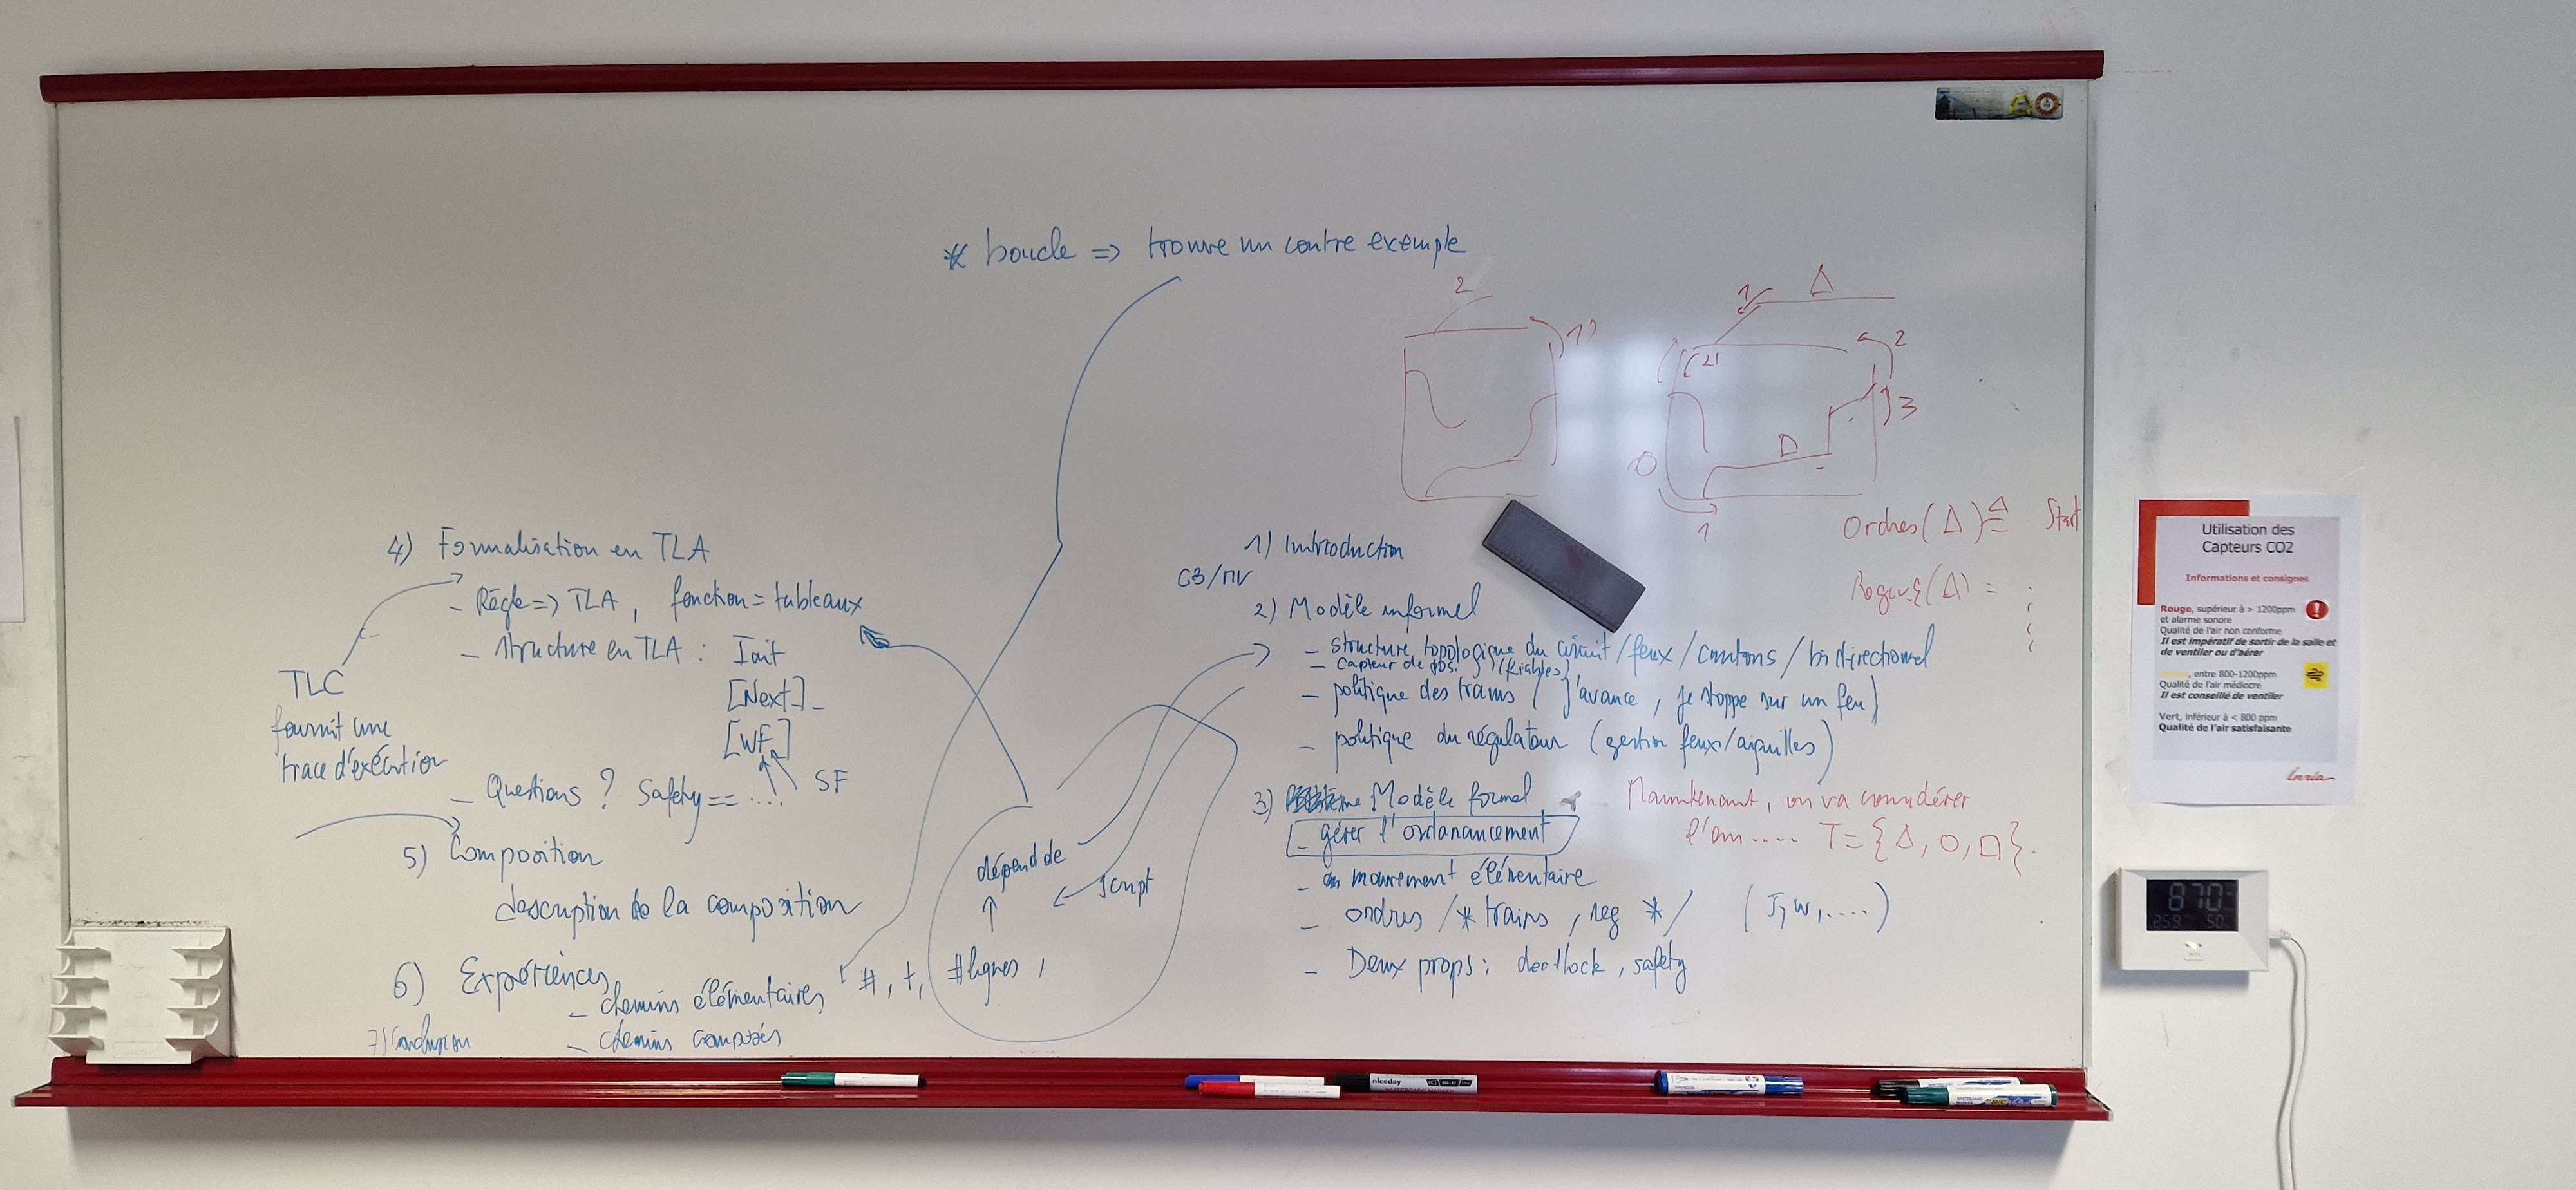
\includegraphics[scale=0.1]{img/sommaire_tableau.jpg}


\bibliographystyle{splncs04}
\bibliography{refs}
\end{document}
